\documentclass[a4paper]{article}
\usepackage{graphicx}
\usepackage{url}
\usepackage{onecolpceurws}
\usepackage[utf8]{inputenc}

\title{Collaboration Networks in Software Development: Perspectives from Applying different Granularity Levels using Social Network Analysis - Research in Progress}

\author{
Miguel Ángel Fernández, Gregorio Robles \\ GSyC/LibreSoft \\
                Universidad Rey Juan Carlos \\ \{ma.fernandezsa@alumnos., gregorio.robles@\}urjc.es
\and
Jesús M. González Barahona \\ Bitergia \\
                jgb@bitergia.com
}

\institution{}


\begin{document}
\maketitle

\begin{abstract}
This paper shows research in progress in the analysis of collaboration networks
found in software development projects. Traditionally, collaboration networks
are obtained by analyzing collaboration in the same file or module/directory;
when two developers perform modifications on the same entity during a given time
period it is assumed that they are at least implicitly collaborating. In our 
research, we want to study how the granularity of the software artifact affects
the research output of collaboration graphs. In this regard, we obtain traditional
graphs based on collaboration in files and augment it with information of
collaboration at the function/method level. In the future we want to include
developer affiliation information to perform a collaboration analysis at the
company level.
\end{abstract}
\vskip 32pt


\section{Introduction/Motivation}

The development of large software systems is a collaborative task where
many developers, sometimes up to thousands of them, are involved. In such 
scenario, software engineering research has been long looking after
understanding how these collaborations arise, and how they evolve over time~\cite{minto2007recommending,singh2010small,surian2010mining,hossain2009social}.

In order to identify collaboration, many scholars have used techniques such as
social network analysis, where two developers (nodes) are connected if they
have collaborated together~\cite{madey2002open,lopez2004applying}. In most social network studies the
resulting network is based on file-based or module-based data of interactions;
if there has been a collaboration between two developers in a file or a module,
these developers are connected. 

Our research is concerned with the fact that the resulting network graph depends
heavily on the granularity level that is selected~\cite{howison2012validity}. When there are tens of files
in a module/directory or thousands of lines in a file, did collaboration really
exist?

Therefore, in addition to the existing collaboration graphs, we have been working
to obtain a new one that takes collaboration at the function/method level into
account. In this type of graph, two developers collaborate if they have modified
the same function in a given time period. We think that, although there might
be exceptions with large functions/methods, this provides a new, still unknown
level of granularity in the analysis that can help to obtain a better global 
picture.

\section{Methodology}

Our methodology studies registered changes made to a given repository tracked by
a versioning system (in our case \texttt{git})\footnote{The tool is available on-line as free software in a GitHub repository: \url{https://github.com/LibreSoftTeam/R-SNA}}. 
From that repository, it extracts the log for a specified date range. Using
that data, the program iterates for each commit, performs a checkout
and uses \texttt{ctags} with each file to identify function/method information
in each of those files.

Next, matches between the commits information and \texttt{ctags} data
(still for each checkout) are searched for, to identify those methods that have
changed. By now, changes in methods are only tracked if the method has not 
changed its name. Future versions of our tool will include heuristics to analyze
as well those functions whose name change.

While changes to functions/methods are extracted, the developers who have performed
these changes are attached to the change. As by now, we do not apply developer merging
algorithms, so that a developer with different aliases will only appear once,
but we plan to do it in the future. This data is aggregated and offered
in two CVS-formatted files, one for collaborations occurring in the same file
and another one with collaborations in the same function/method. This output
can be used by traditional programs to obtain a social network graph, such as
Gephi, or to calculate social network measures and properties.

\section{Case study}

We have used the program to study the evolution of the GNOME-text editor \texttt{gedit}\footnote{The repository of \texttt{gedit} used in this analysis is \url{https://github.com/GNOME/gedit}}.
The considered date range for this study goes from the very beginning of
the project (at least, from the moment a first commit has been found in the log), which is April
15, 1998 until April 15, 2015.
Within this time range, we have chosen time-lapses of six months so
we can handle and understand better the resulting data and its evolution
over time. The chosen time period is consistent with the release period of GNOME 
(at least from 2005 onwards).

In this paper we show the results for two selected timeframes: from January 1, 2001 to May 31, 2001 and from June 1, 2014 to December 31, 2014. For both ranges we offer a graphic representation of collaboration networks between
developers. Each node represents a developer, and edges represents
interactions between them. We have two different graphs for each date range: an in-file collaboration network (developers who have modified same file) and an in-method
collaboration network (developers who have modified same method).

Figure~\ref{fig:2001} shows the different graphs (in-file and in-method data) for the
first half of 2001. As expected the number of collaborations (only those developers
who collaborate are shown in the graph) is larger in the in-file network than in
the in-method one.

\begin{figure}[h!]
\begin{center}
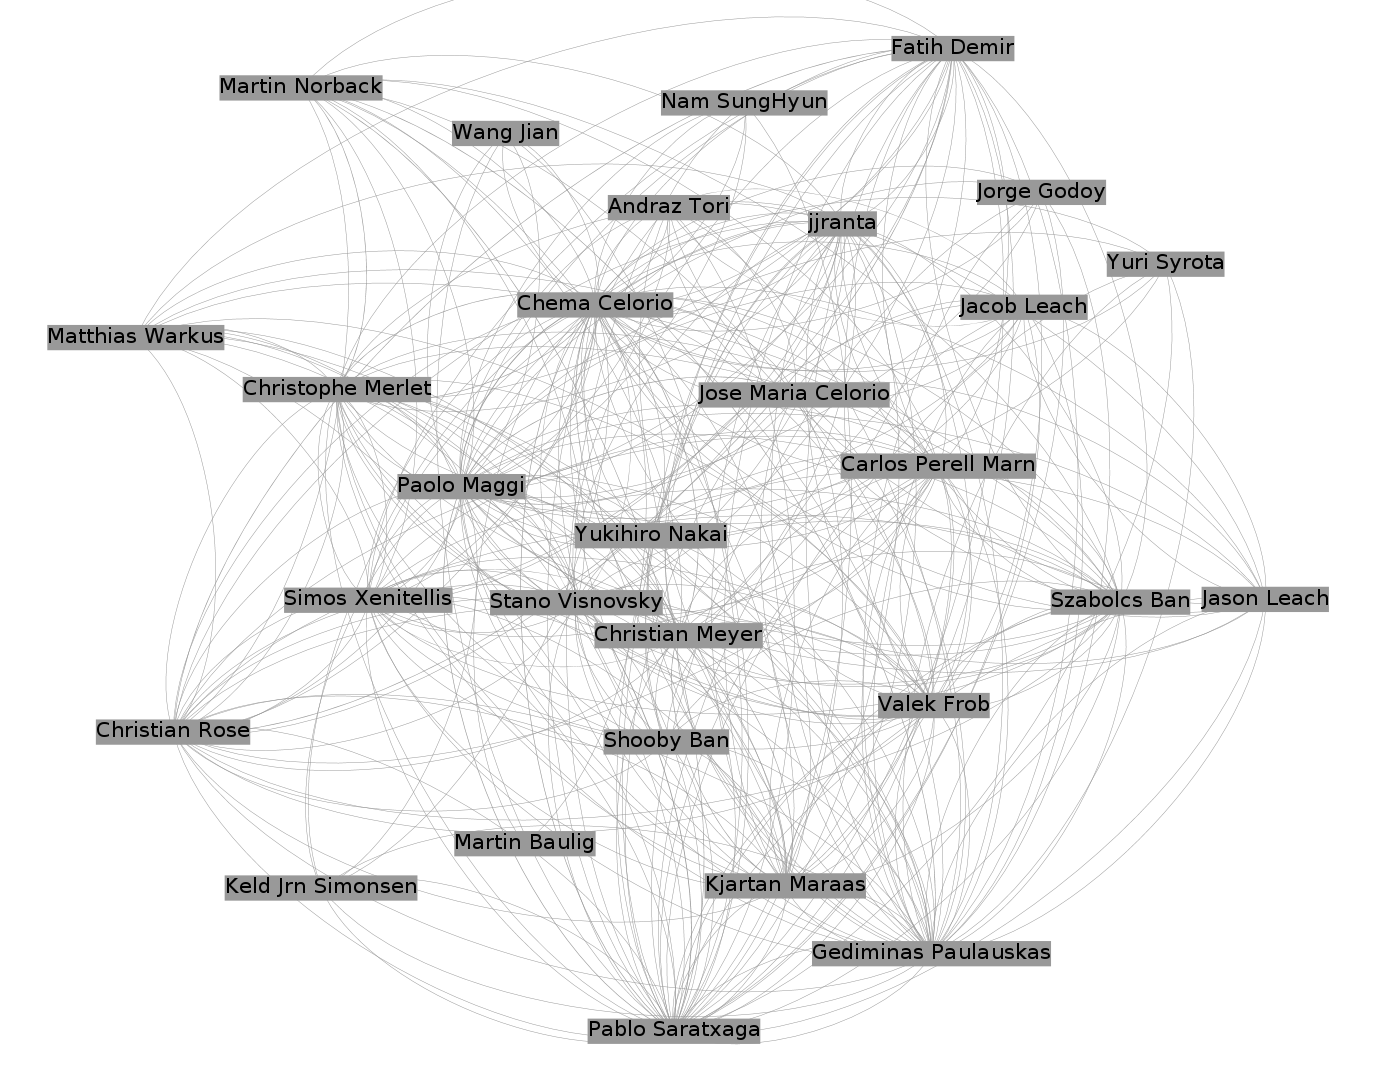
\includegraphics[scale=0.17]{g2001files.png} 
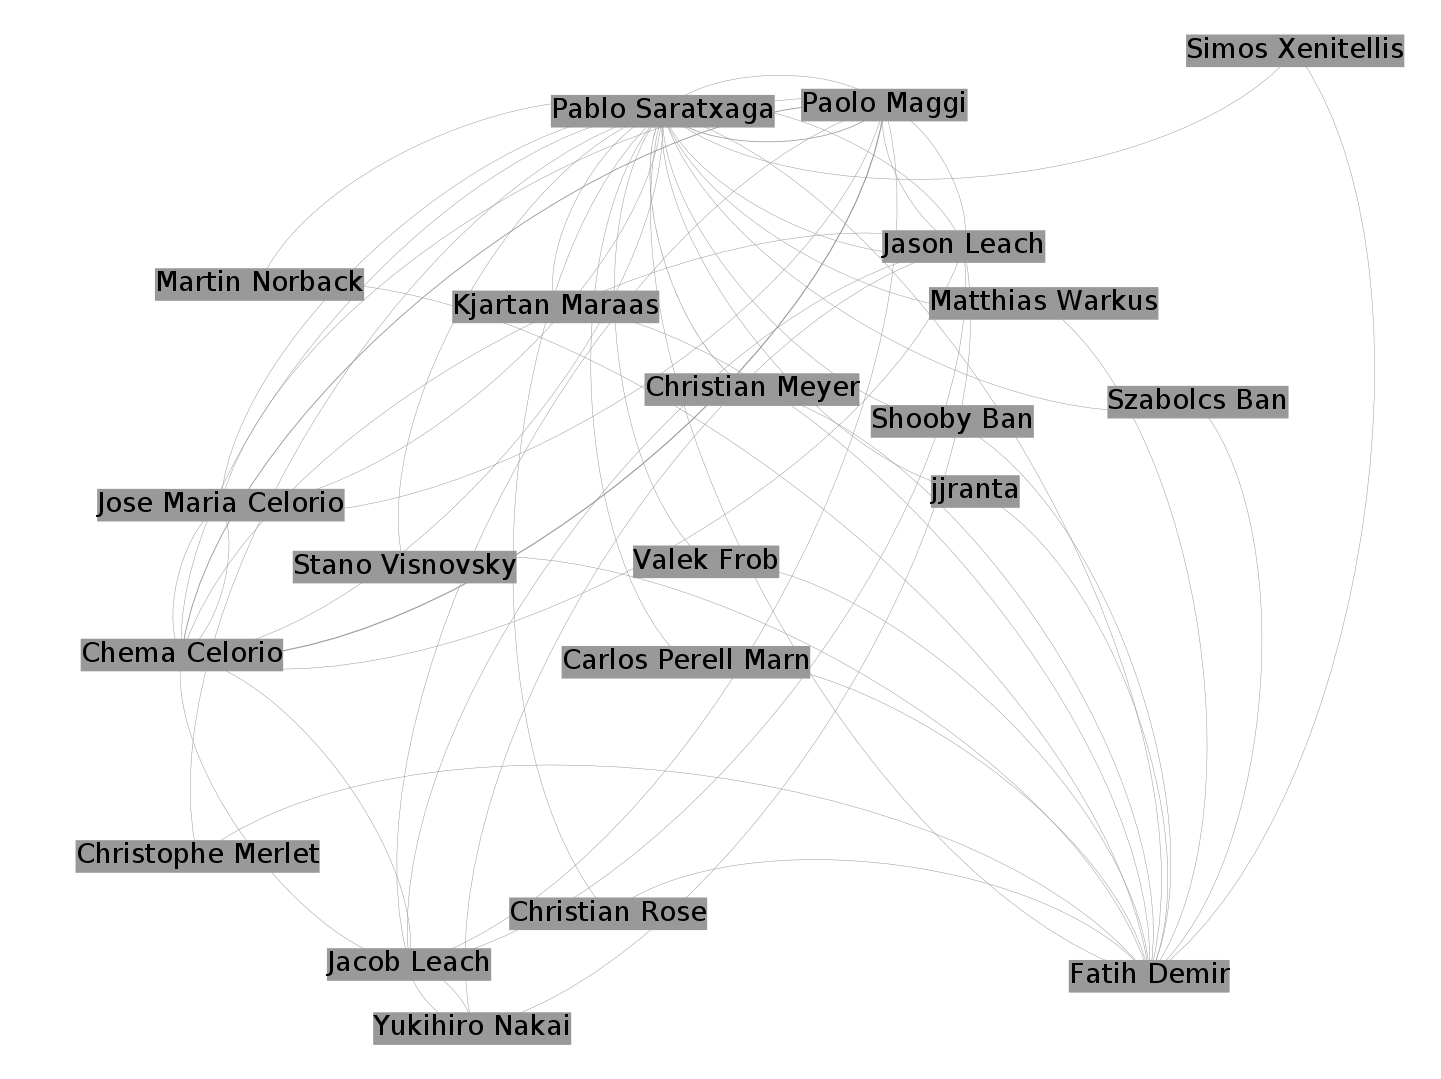
\includegraphics[scale=0.17]{g2001methods.png}
\caption{In-file (left) and In-method (right) collaboration graphs - 2001}
\label{fig:2001}
\end{center}
\end{figure}

Figure~\ref{fig:2014} shows graphs (in-file and in-method data) for the
second half of 2014. We see that the number of contributors to \texttt{gedit}
has grown, and as such its network size and number of collaborations. 

\begin{figure}[h!]
\begin{center}
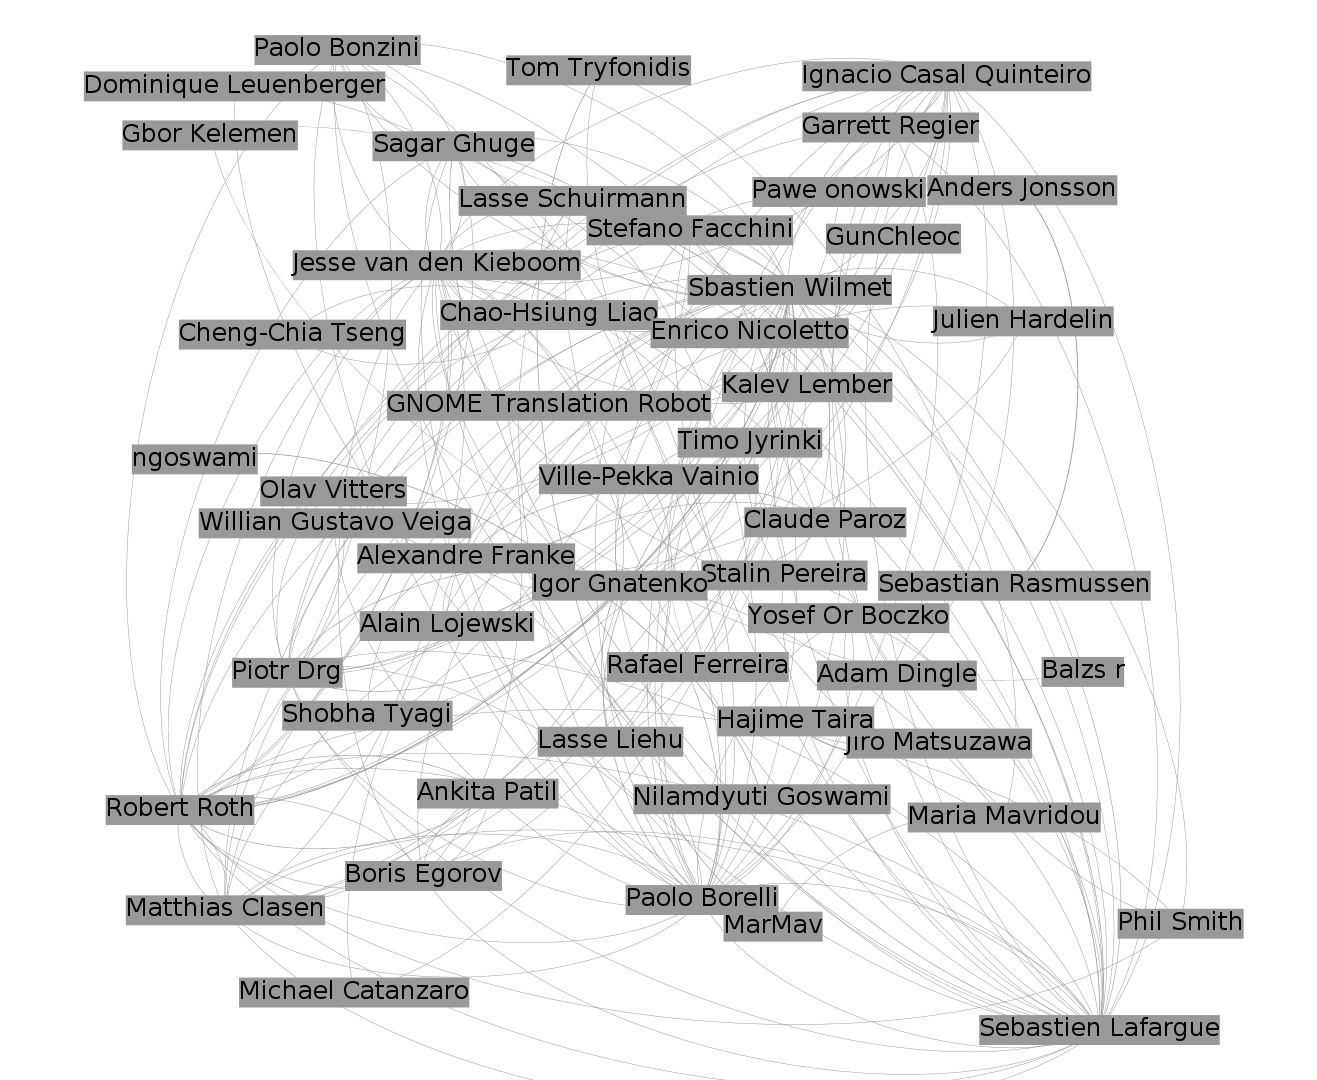
\includegraphics[scale=0.17]{g2014files.png} 
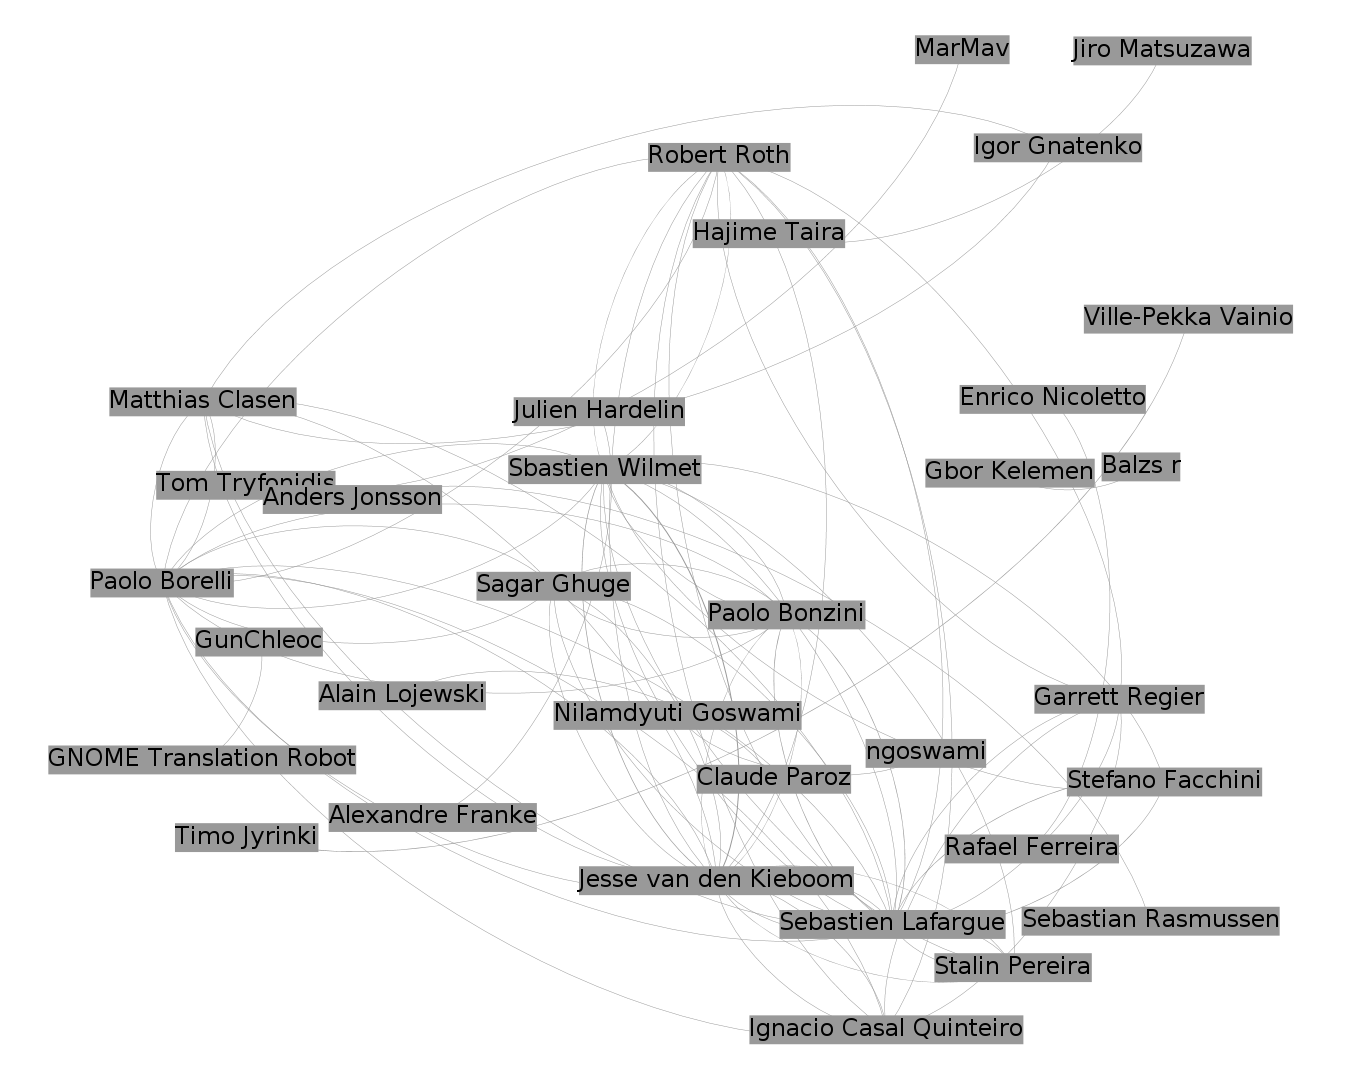
\includegraphics[scale=0.17]{g2014methods.png}
\caption{In-file (left) and In-method (right) collaboration graphs - 2014}
\label{fig:2014}
\end{center}
\end{figure}

We have computed a numerical representation, the betweenness centrality of a node,
that reflects the amount of control that
this node exerts over the interactions of other nodes in the network. 
The values of betweenness given in Tables~\ref{tab:2001} and Table~\ref{tab:2014} 
are normalized, and only nodes that have at least one non-zero value are shown.

As it can be seen the values are very different when considering the two types
of collaboration networks, suggesting that developers that with traditional
techniques (i.e., collaboration in files) may not be that central if collaboration
at the function/method level is considered. This can be observed by ranking 
developers by their betweenness value for both networks; those who are highly
ranked at the file level have not to be the ones that have the higher values
at the function level.

\begin{table}[ht]
\begin{center}
\caption{Normalized betweenness centrality for the first half of 2001.}
\label{tab:2001}
\bigskip
\begin{tabular}{|l|c|c|c|c|}
\hline
Node & Files & Methods/Functions & Rank Files & Rank Methods/Functions \\ \hline
Gediminas Paulauskas & 0.08305 & 0 & 1 & - \\
Chema Celorio & 0.19019 & 0.02140 & 2 & 3 \\ 
Paolo Maggi & 0.12273 & 0.02140 & 3 & 3 \\
Pablo Saratxaga & 0.10483 & 0.23965 & 4 & 1 \\
Jacob Leach & 0.00159 & 0.00737 & 5 & 5 \\
Jason Leach & 0.00159 & 0.06807 & 5 & 2 \\
\hline
\end{tabular}
\end{center}
\end{table}

\begin{table}[ht]
\begin{center}
\caption{Normalized betweenness centrality for second half of 2014}
\bigskip
\label{tab:2014}
\begin{tabular}{|l|c|c|c|c|}
\hline
Node & Files & Methods/Functions & Rank Files & Rank Methods/Functions  \\ \hline
Sebastien Wilmet & 0.14896 & 0.00842 & 1 & 5 \\ 
Sebastien Lafargue & 0.05861 & 0.03879 & 2 & 1   \\
Paolo Borelli & 0.04775 & 0.01284 & 3 & 4 \\
Robert Roth & 0.03033 & 0.00410 & 4 & 6 \\
Jesse van den Kieboom & 0.02957 & 0.01990 & 5 & 3 \\
Piotr Drg & 0.02797 & 0 & 6 & - \\
Ignacio Casal Quinteiro & 0.02728 & 0.00134 & 7 & 7 \\
Boris Egorov & 0.00645 & 0 & 8 & - \\
Matthias Clasen & 0.00832 & 0.02218 & 9 & 2 \\
Alexandre Franke & 0.00061 & 0 & 10 & - \\
Igor Gnatenkov & 0.00027 & 0 & 11 & - \\
\hline
\end{tabular}
\end{center}
\end{table}


\section{Future work}

As future work, we plan to improve our tool with state-of-the art 
functionality by (1) including algorithms to track function name changes~\cite{godfrey2005using}, and (2) integrating algorithms to merge developer aliases~\cite{kouters2012s}.

Once this is done we want to perform several analysis to compare the 
collaboration graphs obtained by analyzing at the file \emph{vs.} the function/method
level, and to see the implications of doing the analysis at a finer level of
granularity. Therefore we want to reproduce some of the studies done in the past that 
have been done at the file level.

In addition, we plan to augment the analysis with developer affiliation information~\cite{gonzalez2013understanding}. This will allow to gain further understanding of 
emerging communities such as OpenStack or WebKit, that are mainly composed of
industrial partners.

\section*{Acknowledgments}

This work has been funded in part by the Spanish Gov. under SobreSale (TIN2011-28110) and by the Comunidad de Madrid under ``eMadrid - Investigaci\'on y Desarrollo de tecnolog\'ias para el e-learning en la Comunidad de Madrid'' (S2013/ICE-2715).

\bibliographystyle{alpha} 
\bibliography{bib}
%inline the .bbl file directly for mailing to authors.

%\begin{thebibliography}{Com79}
%
%\bibitem[Com79]{Comer-btree}
%D.~Comer.
%\newblock The ubiquitous b-tree.
%\newblock {\em Computing Surveys}, 11(2):121--137, June 1979.
%
%\bibitem[Knu73]{Knuth-vol3}
%D.~E. Knuth.
%\newblock {\em The Art of Computer Programming -- Volume 3 / Sorting and
%  Searching}.
%\newblock Addison-Wesley, 1973.
%
%\end{thebibliography}

\end{document}


